% Nicholas Vanderweit
% Fiona Pigott
% Krishan Patel

% Fourier final project--Digital signal processing
% Dec 7 2012

% Set up the layout
\documentclass[12pt]{article}
\usepackage[margin=1in]{geometry}
\geometry{letterpaper}
\usepackage{amssymb}
\usepackage{amsmath}
\usepackage{verbatim}
\usepackage{setspace}
\usepackage{algorithmic}
\usepackage{graphicx}
\usepackage{float}
\usepackage{hyperref}

\newcommand{\inftyint}{\int_{-\infty}^{\infty}}

% Title
\title{Frequency Division Multiplexing \\Using the Fast Fourier Transform }
\author{Nicholas Vanderweit \\Fiona Pigott \\Krishan Patel \\ \\APPM 4350 --
        Fourier Analysis \\Harvey Segur}
\date{\today}

\begin{document}
\maketitle

% Begin  the write-up

% Abstract
\begin{abstract}

The discrete Fourier transform, or DFT, is undoubtedly one of the most
important and widely used operators in signal processing. Because it is
able to represent many common kinds of signals without loss of information, and
because there are many efficient algorithms (called fast Fourier transforms, or
FFTs) to implement it on conventional hardware, the DFT has become an
invaluable tool for analysing and manipulating the frequency information in
digital signals. In this paper, we will investigate Frequency-Division
Multiplexing, one such application which focuses on sending several signals
concurrently in time through a fixed-bandwidth channel, by translating each of
the constituent frequencies into its own allocation within the channel. In the
process, we will investigate the relationship between the DFT, the DTFT
(discrete-time Fourier transform), and the Fourier transform on an infinite
continuous domain.


\end{abstract}

\clearpage

\section{Mathematical Formulation \\of Digital Signal Processing}

\subsection{Nyquist-Shannon Sampling Theorem}

One of the most important results in signal processing, the Nyquist-Shannon
Sampling Theorem (often simply the Nyquist Sampling Theorem) helps to develop
the Discrete Fourier Transform. The result of this theorem is that any periodic
signal can be represented by a discretly sampled set of points, with samping 
frequency greater than the largest frequency present in the signal. 

\subsubsection{Proof}

The following proof of the Sampling Theorem is an adaptation of Shannon's original
proof, found in \emph{Boundary Value Problems and Partial Differential 
Equations} by David L Powers.

Assume the function \(f(t)\) is some infinite function in the time domain, but note that
this proof holds as well for a spacial \(f(x)\).

A signal \(f(t)\) is called \emph{band limited} if its Fourier transform is
identically zero except in a finite interval.  \[\hat{f}(\omega) \equiv 0 \quad
\forall \, \omega \; \text{s.t.} \; |\omega| > \Omega \text{ ``cutoff
frequency"}\] i.e., the signal is composed of a limited number of frequencies.
Practically, most signals that are not completely random are band limited.

If \(f(t)\) is band limited: \begin{equation} \label{eq:nft} f(t) = \inftyint
    \hat{f}(\omega)e^{i\omega t} \,d\omega \; = \; \int_{-\Omega}^{\Omega}
    \hat{f}(\omega)e^{i\omega t} \,d\omega \end{equation}

Now, since \( \hat{f}(\omega) \) is defined on a finite, rather than an
infinite, interval, \( \hat{f}(\omega) \) can be expressed as as a summation
rather than an integral: \[\hat{f}(\omega) = \sum_{n = -\infty}^{\infty}
\hat{c}_{n}e^{\frac{i n \pi \omega}{\Omega}} \] Where the complex coefficients
\( \hat{c}_n\) are the Fourier transform of \( \hat{f}(\omega) \): \[\hat{ c}_n
= \frac{1}{2\Omega} \int_{-\Omega}^{\Omega} \hat{f}(\bar{\omega})e^{\frac{-i n
\pi \bar{ \omega}}{\Omega}}\,d\bar{\omega}\]

Looking at \(\hat{c}_n\), and replacing \( \frac{-n\pi}{\Omega} = \bar{t}\)
yield the definition of the Fourier transform of \( f(\bar{t})\): \[ \hat{c}_n
= \frac{1}{2\Omega} \int_{-\Omega}^{\Omega}
\hat{f}(\bar{\omega})e^{i\bar{\omega}\bar{t}}\,d\bar{\omega} =
\frac{1}{2\Omega} f(\bar{t}) = \frac{1}{2\Omega} f(\frac{-n\pi}{\Omega})\]

\begin{equation} \label{eq:nfhat} \therefore \; \hat{f}(\omega) = \sum_{n =
    -\infty}^{\infty} \hat{c}_{n}e^{\frac{i n \pi \omega}{\Omega}} = \sum_{n =
    -\infty}^{\infty} \frac{1}{2\Omega} f(\frac{-n\pi}{\Omega})e^{\frac{i n \pi
    \omega}{\Omega}} = \frac{1}{2\Omega} \sum_{n = -\infty}^{\infty}
    f(\frac{n\pi}{\Omega})e^{-i \omega \frac{n \pi}{\Omega} } 
\end{equation}

Therefore, the Fourier transform can be completely determined by taking
discrete samples of the function \( f(t) \) at only times t = \(
\frac{n\pi}{\Omega}\). Because any function with a Fourier transform can 
always be recovered exactly from its Fourier transform, this implies that the 
band limited function \( f(t)\) can be completely determined by the same 
discrete set of samples.

Use \eqref{eq:nft} and \eqref{eq:nfhat} to reconstruct \( f(t)  \):
\begin{equation} \label{eq:ndtft} f(t) = \int_{-\Omega}^{\Omega}
    \frac{1}{2\Omega} \sum_{n = -\infty}^{\infty} f(\frac{n\pi}{\Omega})e^{-i
    \omega \frac{n \pi}{\Omega} } e^{i\omega t} \,d\omega = \frac{1}{2\Omega}
    \sum_{n = -\infty}^{\infty} f(\frac{n\pi}{\Omega}) \int_{-\Omega}^{\Omega}
    e^{-i \omega \frac{n \pi}{\Omega} } e^{i\omega t} \, d\omega \end{equation}

And since the Fourier transform \( \hat{f}(\omega) \) is periodic with a period
of \( 2\pi\), the sampling frequency \( n\) is given by: \[ \frac{n\pi}{\Omega}
= 2\pi \Rightarrow n = 2\Omega\]

Thus, the result of the Nyquist-Shannon sampling theorem: any bandwidth limited
function with the cutoff frequency \( \Omega \) in the time (or spacial) domain
can be reconstructed exactly from samples taken at a rate of \( 2\Omega \).

% This was totally unnecessary to this proof (oops), but I'm going to hang on
% to it for now.  \[  \hat{f}(\omega)  =\frac{1}{2\Omega}  \sum_{n =
% -\infty}^{\infty} f(\frac{n\pi}{\Omega})e^{\frac{-i n \pi \omega}{\Omega}} \]
%
% Note that it is a property of the Fourier transform that: \[
% \mathcal{F}(g(Ct)) = \frac{1}{C} \; \hat{g}(\frac{\omega}{C}) \]
%
% Which is easily shown. Taking the Fourier Transform of \(g(Ct)\) yields: \[
% \mathcal{F}(g(Ct)) = \inftyint g(Ct)e^{-i\omega t} \,dt \] Performing a
% simple u-substitution for \(Ct\), \(u = Ct\): \[u = Ct  \Rightarrow du = Cdt
% \Rightarrow \frac{1}{C} \, du = dt \] \[ \mathcal{F}(g(u)) = \frac{1}{C}
% \inftyint g(u)e^{-i\frac{\omega}{C} u} \,du = \frac{1}{C} \;
% \hat{g}(\frac{\omega}{C}) \]


\subsubsection{Implications}

The Nyquist-Shannon Sampling Theorem is important because it demonstrates how
to use digital processing (which is necessarily discrete) to analyse signals. 

In practice, many signals are only \emph{very nearly} band limited, meaning
that the vast majority of frequencies are under a certain \( \Omega \), but
some almost random noise causes some small frequency components \( \omega \)
with \( |\omega| > \Omega \). The signal might also be artificially band
limited because the sampling frequency \( f_s\) is determined by factors other
than the signal's band (such as limited storage), and so the frequencies \(
\omega \) in the signal are represented faithfully only for \(|\omega| <
\frac{f_s}{2} \). Because samples at \( f_s > 2\Omega \) only correspond to
unique periodic components with frequency \( < \frac{f_s}{2} \), samples from
components with frequency \( > \frac{f_s}{2} \) are aliased to a frequency
components with the same sample with frequency \( < \frac{f_s}{2} \). In both
cases, this aliasing results in noise and distortion of the sound; aliasing is
avoided only by understanding the frequency components of the time dependent
signal. When small sampling frequency cannot be avoided, the added noise from
aliasing can be eliminated by artificially bandwidth limiting the
signal--taking the Fourier transform and setting it equal to zero outside of
some band \( |\omega| > \frac{f_s}{2}  \). This way, information is lost, but
the remaining signal is clearer. 

\begin{figure}[H]
\begin{centering}
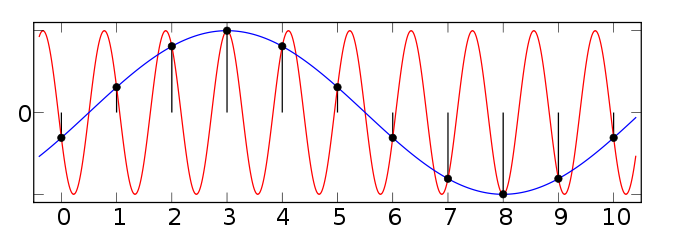
\includegraphics[width=.5\linewidth]{AliasingSines.png}
\caption{A graph showing the effects of aliasing. If the red sine function 
has a frequency \( > \frac{f_s}{2}\), its samples can be mapped to a function
(the blue curve) with a frequency \( < \frac{f_s}{2}\). The blue sine 
function is \emph{aliased} to the \( f_s\) frequency samples of the red sine
function.}
\end{centering}
\end{figure}

% I think some illustration of what aliasing means here (i.e. 2 sine waves with
% the same sample) would be helpful. Remind me to look/ create one.

\subsection{Discrete Fourier Transform}

The Fourier transform of a continuous signal gives a continuous signal. Above,
the proof of the Nyquist-Shannon Sampling Theorem shows how a Fourier transform
of a discrete signal (a discrete time Fourier transfrom) can gives an exact, continuous signal. Finally, the
discrete Fourier transform takes a discrete signal and maps that to a discrete
transform, which, at a high enough sampling frequency, is a set of samples from
the continuous transform.

\subsubsection{Formulation}

The Nyquist-Shannon Sampling Theorem demonstrates that any band limited signal
can be expressed as a discrete time signal. Furthermore, any practical signal
with only periodic components is periodic on some interval. Call that interval
\( T_0\). 

Say that for some sampling frequency \(f_s\), \(T_0 = N\frac{1}{f_{s}} \).
Therefore, one period \( T_0\) can be divided into N intervals with length \(
\frac{1}{f_{s}}\).

We know that the signal \(f(t)\) can be represented as the infinite sum of its
frequency components, with coefficients \(c_n\).

\[ f(t) = \sum_{n = -\infty}^{\infty} \,c_n e^{i\omega t} \] \[ c_{n} =
\frac{1}{T_0} \int_{0}^{T_0} f(t) e^{i\omega t} dt\]

Because we defined \(T_0\) as the period of the function, \(c_{n}(\omega) \)
should have a period of \( T_0\), \(e^{i\omega T_0} = e^{i\omega nT_0}\). Since
\(e^{i x}\) has a period of \( 2\pi \), \( \omega \) must be equal to
\(\frac{2\pi n}{T_0} \). 

\[ \therefore c_{n} = \frac{1}{T_0} \int_{0}^{T_0} f(t) e^{i \frac{2\pi}{T_0} t
} \; dt\] 

Now, using the Left-Hand Riemann sum to approximate \( c_n\) with \( N\)
intervals of \( \frac{1}{f_s} \): \[ c_{n} = \frac{1}{T_0} \frac{1}{f_s} \;
\sum_{k = 0}^{N-1} f(k \frac{1}{f_s}) e^{i \frac{2\pi n}{T_0} k\frac{1}{f_s}}
\]

Which simplifies to: \[ c_{n} = \frac{1}{N} \; \sum_{k = 0}^{N-1} f(k
\frac{1}{f_s}) e^{i \frac{2\pi n}{N}k} \]

Written where \( f(k \frac{1}{f_s}) =\) the indexed sample \(f_k\), spaced
\(\frac{1}{f_s}\) apart, this Riemann sum yields the common form of the
Discrete Fourier Transform (DFT): \[ c_{n} = \frac{1}{N} \; \sum_{k = 0}^{N-1}
f_k \, e^{i \frac{2\pi n}{N}k} \]

And from the discussion of Nyquist sampling frequency above, we know that as
long as \(f_s = 2\Omega\), the signal's DFT will be non-aliased representation
of its continuous Fourier transform.

This proof is founded on idea from Li Tan's book \emph{Digital Signal
Processing} and \emph{Applied Partial Differential Equations} by Richard
Haberman.

\subsubsection{Properties of the Discrete Fourier Transform}

The Fourier transform lends itself well to signal processing because it
provides a radically different way to view the signal while preserving all of
its information. Many signals which are difficult to analyse in the time domain
can be transformed into the frequency domain where they become regular. There
are two important properties of the discrete Fourier transform that are
integral to the digital analysis of real signals: its periodicity and the
\emph{reality condition}.

\subsubsection*{Periodicity}
As to the periodicity of the function, we enforced a period of \(T_0\) on the
discrete Fourier transform in the formulation. This period results directly
from the sampling frequency \(f_s\) with \(T_0 = \frac{N}{f_s}\) (which is
controlled during implementation). That way, when we sample a function (say, a
voice) to analyse it, we know what the period of the transform and of resulting
time domain signal should be, and can select only one period to analyse.

An interesting way of showing the periodic properties of the discrete transform
is to recognize the discrete transform as a special kinda of Dirac delta. 

The Dirac delta is a \emph{sifting function} defined as the derivative of the 
unit step function. By definition, a sifting function samples some other 
function \( f(t) \) at some arbitrary point \( \tau \). The the inner product 
of the Dirac delta (defined below) and \( f(t)\) is equal to \( f(\tau) \):
\[ \inftyint \delta(t - \tau)f(t) \, dt = f(\tau) \]
With that property, with \(n\) Dirac deltas, \( f (t) \) would be sampled
\( n\) times with samples spaced \( \tau\) units apart:
\[ \inftyint \delta(t - n\tau)f(t) \, dt = f(n\tau) \]
Notice that computing the discrete Fourier transform of a continuous 
signal is exactly that--taking \( n = \frac{1}{f_s} \) Dirac deltas, computing 
thier inner products to sample a function \( f(t) \) \(n\) times, then
taking the transform of those samples. For \( |n| \to \infty \), the 
combination of all of these Dirac deltas is called and infinite Dirac comb, 
and the transform of those samples is the transform of the Dirac comb over some
interval. 

This brings us to note a fundamental property of the Dirac comb, which we will
use in our analysis: the frequency of samples that make up the comb, 
\( f_s \), is the inverse frequency of the transform of those samples.
Another way of stating that property is that for some spacing \( \tau\) 
between sample points in the time domain, the spacing in the frequency 
domain is \( \frac{1}{\tau} \). A proof and examples of this can be found in 
the Allen and Mills, as well as the Edinburgh physics depertment references.

The periodicity of function and transform stated above, which we rely to analyze 
signals in our implementation of Frequency Division Multiplexing,
results directly from the above property of the Dirac comb.

\subsubsection*{Reality Condition}
The second property that we mape use of in manipulating signals, the reality
condition, holds for all Fourier transforms, and the reality condition states
that for all Fourier transforms of all real-valued functions: \[\hat{f}(\omega)
= \overline{\hat{f}(-\omega)} \]

Which can be easily demonstrated.  Recall Euler's identity: \(e^{ix} = cos(x) +
i\,sin(x)\) and make note of the fact that \(cos(x)\) is even: \(cos(x) =
cos(-x)\), and that \(sin(x)\) is odd: \(sin(-x) = -sin(x)\).  Then the Fourier
transform definition: \[ \hat{f}(\omega) = \inftyint f(t)e^{-i\omega t} \,dt =
\inftyint f(t)(cos(\omega t) - i\,sin(\omega t)) \, dt = \inftyint
f(t)cos(\omega t)\,dt \,- \,i\inftyint f(t)sin(\omega t) \, dt\] \[
\hat{f}(-\omega) = \inftyint f(t)e^{i\omega t} \,dt = \inftyint f(t)(cos(\omega
t) + i\,sin(\omega t))\,  dt= \inftyint f(t)cos(\omega t)\,dt \,+ \,i\inftyint
f(t)sin(\omega t) \, dt\] \[ \therefore \hat{f}(\omega) =
\overline{\hat{f}(-\omega)} \]

\subsection{Fast Fourier Transform}
As it is formulated, the discrete Fourier transform has a time complexity of
\(O(n^2)\), because each of the \(n\) output samples requires a summation over
all \(n\) input samples. This is similar to the problem of sorting: a na\"{i}ve
solution requires making a computation using every element of the input, for
each element of the input.

Like the sorting problem, the DFT has considerably more efficient ``divide
and conquer'' algorithms like the Cooley-Tukey algorithm, which reduce the
time complexity to \(O(n \log{n})\) by recursively breaking the DFT into
subproblems. The Cooley-Tukey FFT over \(N\) elements factors \(N\) to express
the DFT as a combination of several DFTs on smaller inputs. This algorithmic
speedup greatly enhances the feasibility of using the DFT on large data sets.

\section{Frequency Division Multiplexing}

\subsection{Our Implementation}
To simulate transmitting multiple signals over a channel of a fixed bandwidth,
we created a simulation using GNU Octave (a free and open source
MATLAB\textsuperscript{\textregistered} clone) which reads in two
single-channel WAV files sampled at some frequency \(f_s\) and performs the
necessary modulation to place them in adjacent band allocations, each \(f_s/2\)
Hz wide.

To accomplish this, we first take the Fourier transform of each signal. This
gives us a complex-valued vector of the same length. Since the signal is real,
the aforementioned reality condition holds and we can safely discard the
negative frequencies without losing any information. At this point, there is
a simple way to combine the remaining frequencies: we simply concatenate them.
By concatenating the signals, we move the translated signal into the higher 
portion of the frequency band. This is called modulating the signal.

\begin{figure}
    \caption{The first input sample in time}
    \centering
        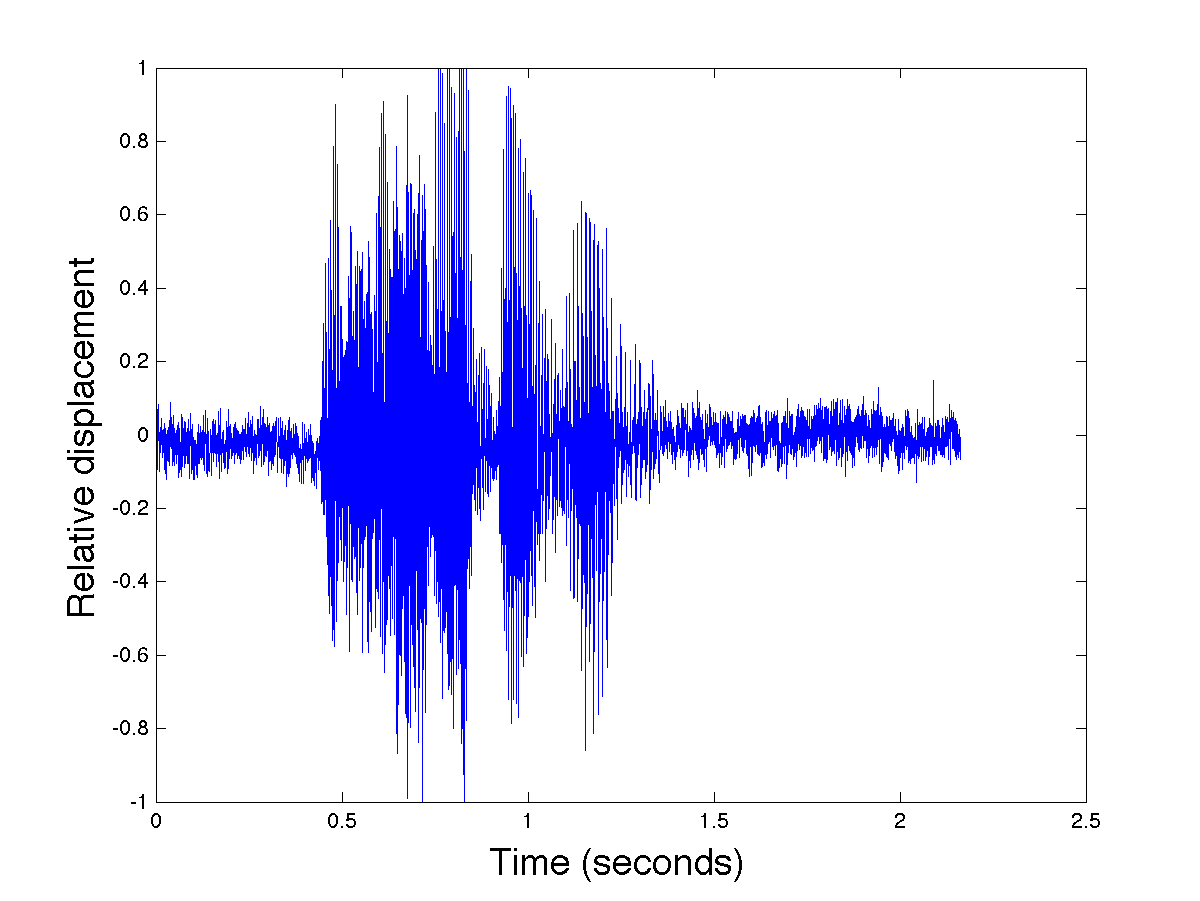
\includegraphics[width=0.7\textwidth]{sample1-orig.png}
\end{figure}

\begin{figure}
    \caption{The second input sample in time}
    \centering
        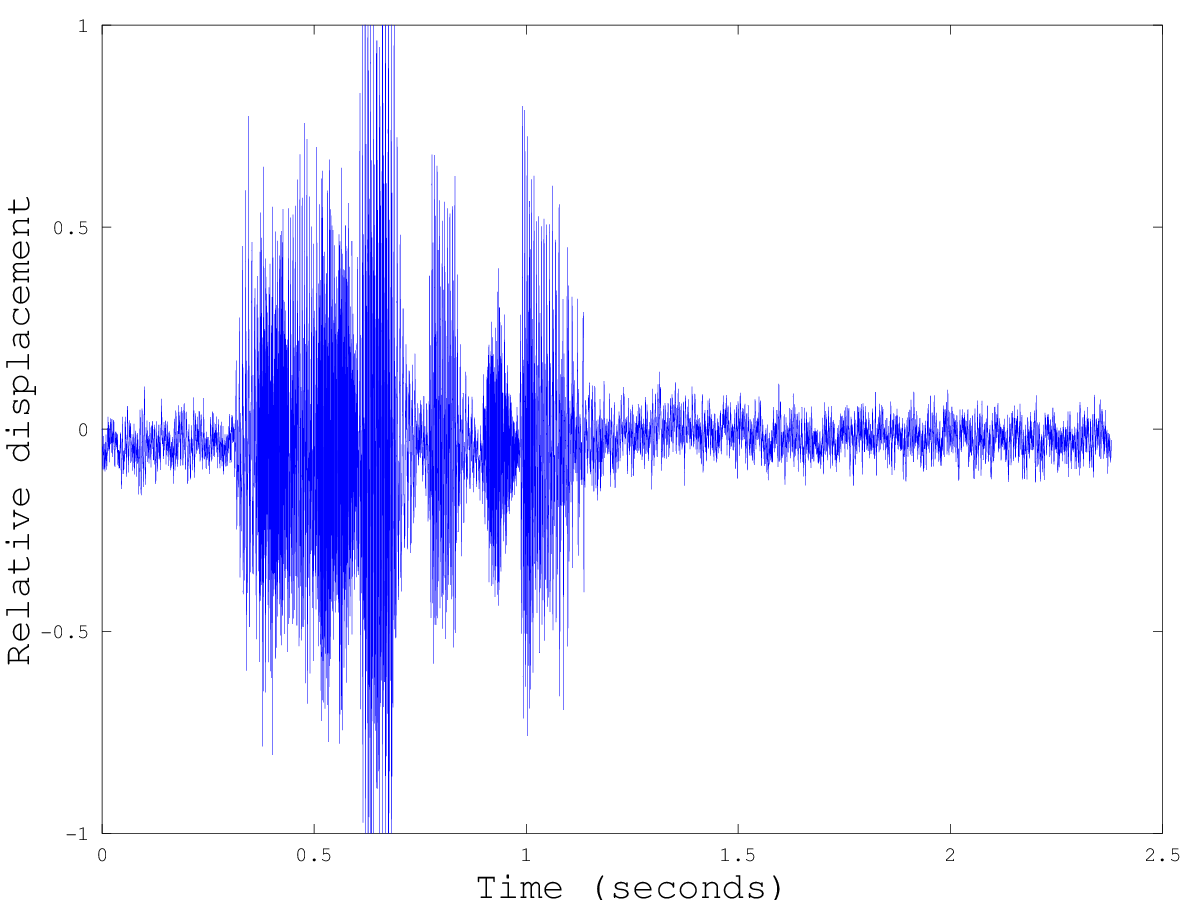
\includegraphics[width=0.7\textwidth]{sample2-orig.png}
\end{figure}

\begin{figure}
    \caption{The first input sample in frequency}
    \centering
        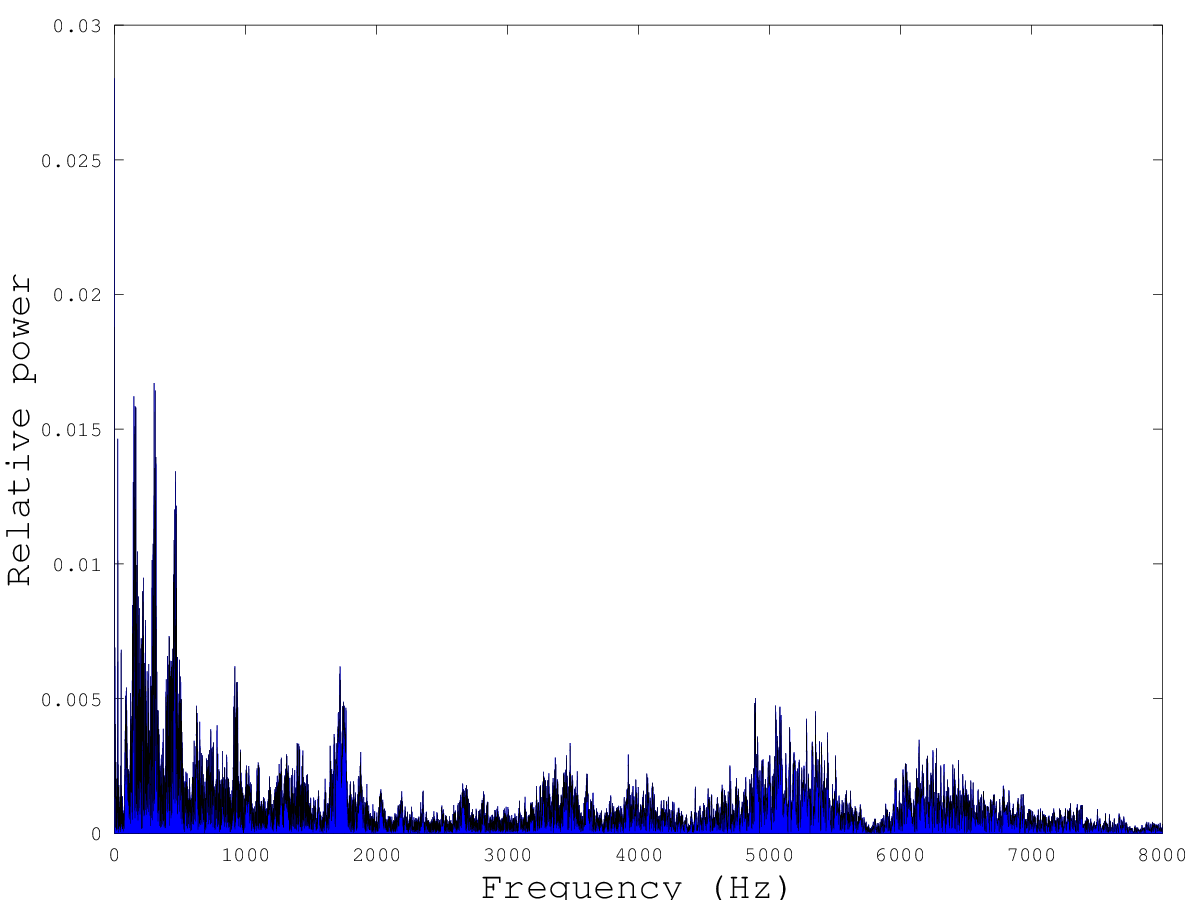
\includegraphics[width=0.7\textwidth]{spectrum1-orig.png}
\end{figure}

\begin{figure}
    \caption{The second input sample in frequency}
    \centering
        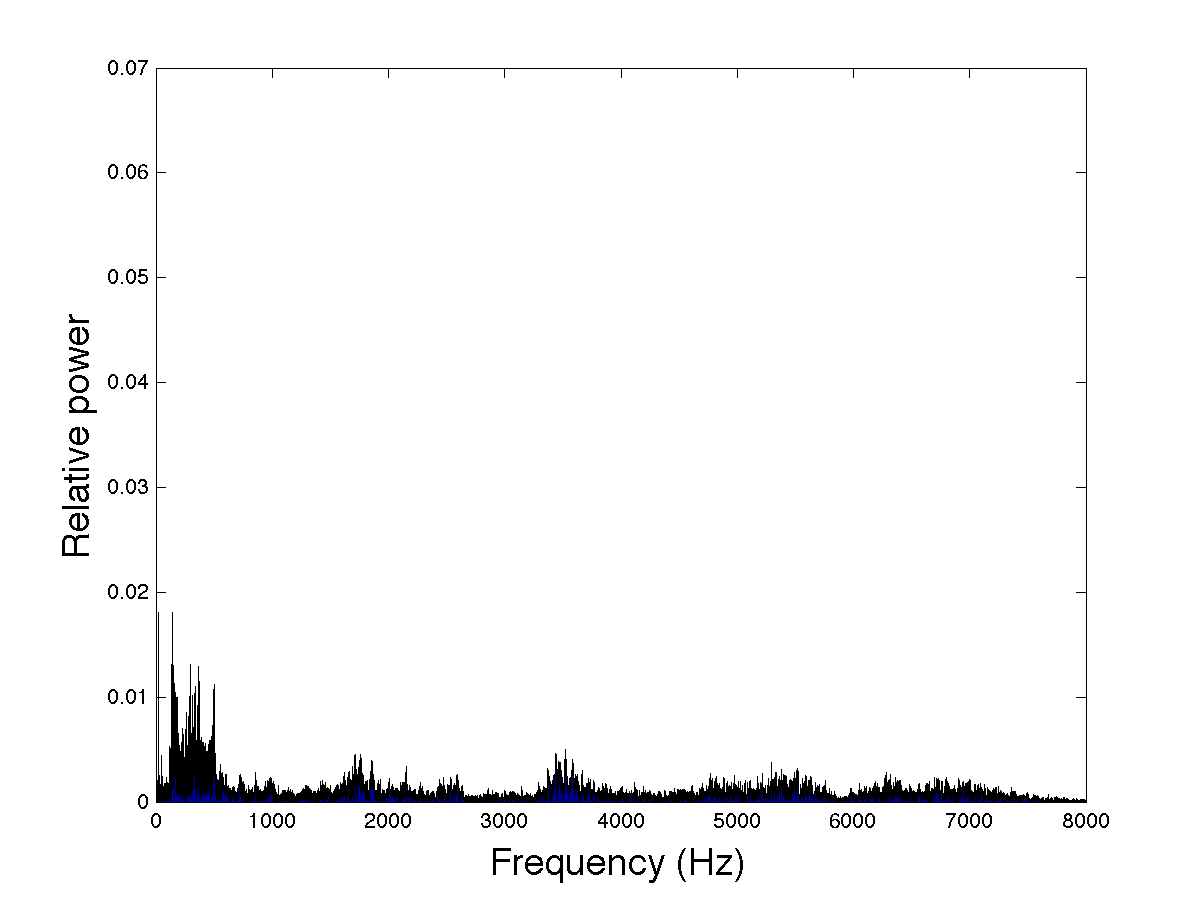
\includegraphics[width=0.7\textwidth]{spectrum2-orig.png}
\end{figure}

\begin{figure}
    \caption{The modulated output in frequency}
    \centering
        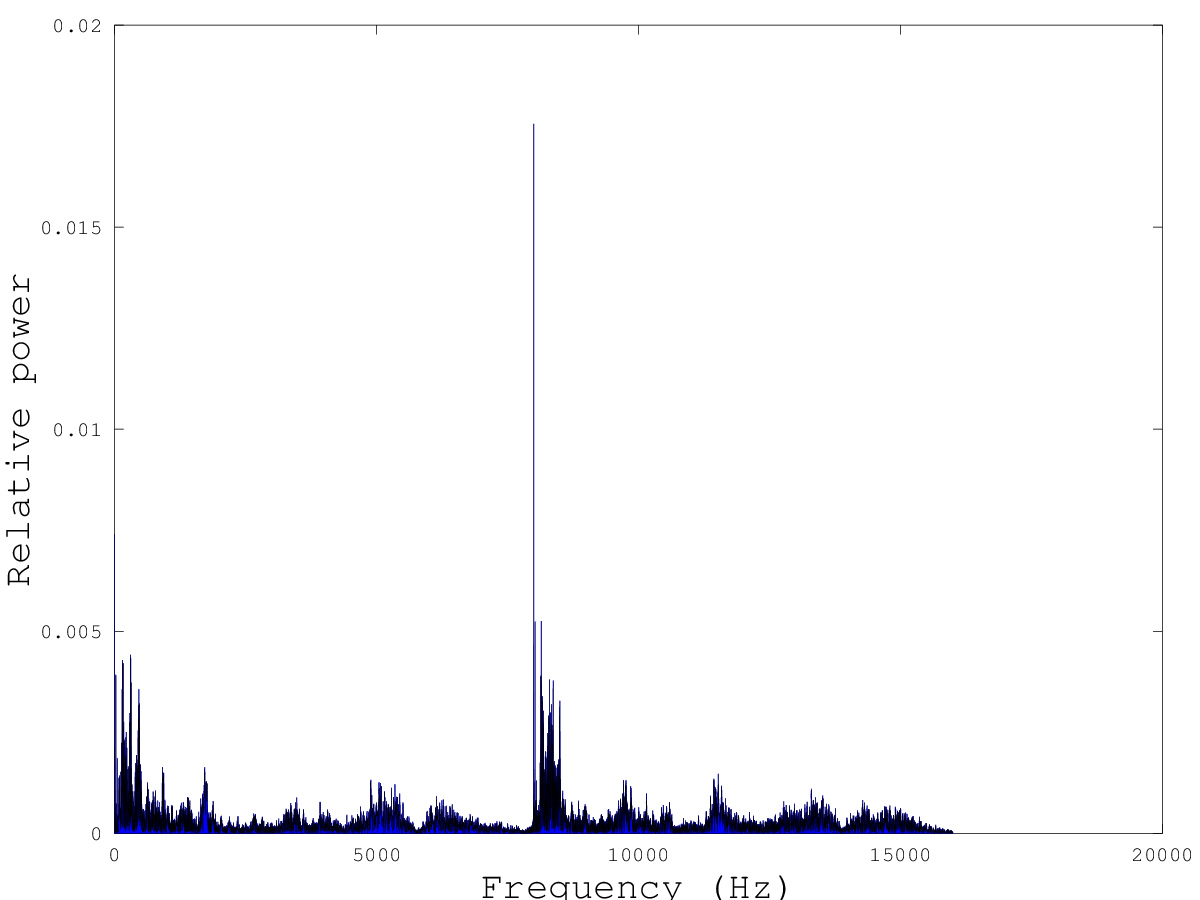
\includegraphics[width=0.7\textwidth]{spectrum-stacked.png}
\end{figure}

\begin{figure}
    \caption{The modulated output in time}
    \centering
        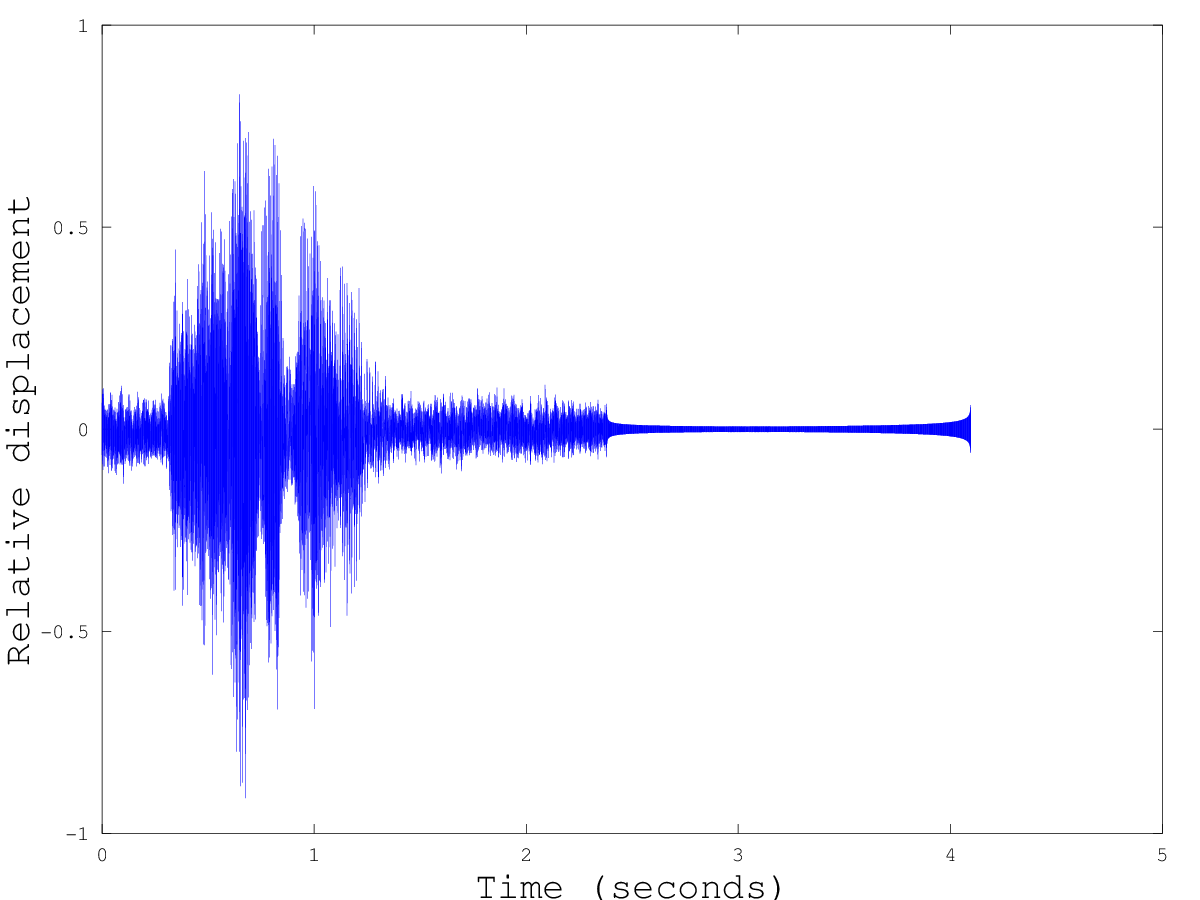
\includegraphics[width=0.7\textwidth]{stacked.png}
\end{figure}
Finally, to satisfy the reality condition, so that the inverse FFT of these
new frequencies is real, we generate the negative frequencies by appending
the reverse of the complex conjugate of the positive frequencies. Taking the
inverse FFT, we now have a periodic signal with all of the frequency
information of each input signal, and which is twice as long. Hence it must
be sent at twice the input sampling frequency in order to maintain the same
time scale. This is equivalent to saying that it must be sent over a channel
which is wide enough to accommodate both signals, by the Nyquist theorem.

To demodulate these signals, the Octave code takes the FFT of the modulated
signal. At this point, it is simply a process of stripping away the redundant
frequency information and splitting the frequency vector in half to reveal
the information contained in each of the individual signals. We then
replicate the negative frequencies as before, and use the inverse FFT to
recover the input signals.

\subsection{A Broader Perspective}
Frequency division multiplexing (FDM) is a method of sectioning the large
frequency band of a medium into non-overlapping frequency sub-bands, each of
which contains a separate signal.

One could fathom a scheme for multiplexing in which the samples in time from
each signal are sent one after another. In a certain sense, this sequencing
is analogous to what is done in our implementation. The difference is that,
instead of sequencing the signals in \emph{time}, we sequence them in
\emph{frequency}. That is, instead of each occupying a separate portion of the
time domain, each signal takes up a distinct portion of the frequency domain.
The Fourier transform gives an excellent lens to describe processes on
frequencies in terms of familiar problems in time and spacial domains.

A good example of the FDM process is the telephone system. When a person talks
on a telephone the audio signal is bandwidth limited and with multiple phones
there are multiple audio signals with similar bandwidths. If a telephone
wire were to send only one signal in each transmission then most of the
medium’s bandwidth would be wasted. Instead FDM translates some of the signals
(modulation) into different frequency sub-bands so that multiple signals can be
sent in one transmission. When the transmission is received then the signals
are inversely translated (demodulation) into their original forms and audio
frequencies used by humans.

Similarly, the modern notion of a digital subscriber line uses existing
telephone infrastructure to provide high-speed internet. This works by encoding
digital data in higher frequency portions of the band, and using filters to
keep voice and digital data separate. Radio transmissions is
a usage of FDM: various agencies including the Federal Communications Commission
and International Telecommunications Union set limits on bands for various
channels, and operators transmit within a small portion of the frequency spectrum.

\clearpage
\section{Extension of Principles}

The same properties of real signals and Fourier analysis that make Frequency 
Division Multiplexing feasible lend themselves to other real-world application;
indeed, the unique interplay between time/ spacial domains and the frequency
domain forms the basis for the mathematics behind hundreds of software, engineering,
and science applications.

The idea that most audio or visual signals are bandwidth limited (or, at least,
human perception is bandwidth limited) becomes file compression and efficient
transmission. 

Recent experimentation with signal tranmission, including using 
different wavelength lasers to send multiple signals over one fiber optic cable,
makes use of fast digital modulation and demodulaton of signals using the FFT.

Analysing light signals in the frequency domain has long helped to identify 
chemicals in spectroscopy. Now, converting sounds and images into the frequency 
domain helps researchers to identify materials, chemicals, distinct voices, and 
detect edges.

Converting audio signals into the frequency domain and then frequency-shifing 
those signals gives us synthesizers and auto-tuners; selecting for and 
changing only certain frequencies in image manipulation software gives us 
color and sharpness filters.


\section{Conclusions}

\section{Works Cited}
``Aliasing." Wikipedia. Wikimedia Foundation, 12 Sept. 2012. Web. 09 Dec. 2012
\vspace{0.3 cm} \noindent \hangindent = 0.6 cm \hangafter = 1 {Allen, Ronald
L., and Duncan W. Mills. Signal Analysis: Time, Frequency, Scale, and
Structure. Piscataway, NJ: IEEE, 2004. Print.}

\vspace{0.3 cm} \noindent \hangindent = 0.6 cm \hangafter = 1 Haberman,
Richard. Applied Partial Differential Equations: With Fourier Series and
Boundary Value Problems. Upper Saddle River, NJ: Pearson Prentice Hall, 2004.
Print.

\vspace{0.3 cm} \noindent \hangindent = 0.6 cm \hangafter = 1 Powers, David L.
Boundary Value Problems: And Partial Differential Equations. Amsterdam:
Elsevier/Academic, 2010. Print.

\vspace{0.3 cm} \noindent \hangindent = 0.6 cm \hangafter = 1 School of
Phyiscs. "The Fourier Transform (What You Need to Know)." The University of
Edinburgh, 10 Sept. 2007. Web. 9 Dec. 2012.
\url{http://www2.ph.ed.ac.uk/~wjh/teaching/Fourier/documents/booklet.pdf}

\vspace{0.3 cm} \noindent \hangindent = 0.6 cm \hangafter = 1 Tan, Li. Digital
Signal Processing: Fundamentals and Applications. Amsterdam: Academic, 2008.
Print.

\vspace{0.3 cm} \noindent \hangindent = 0.6 cm \hangafter = 1 Weinstein, S.;
Ebert, P.; , "Data Transmission by Frequency-Division Multiplexing Using the
Discrete Fourier Transform," Communication Technology, IEEE Transactions on ,
vol.19, no.5, pp.628-634, October 1971
\url{http://ieeexplore.ieee.org/stamp/stamp.jsp?tp=&arnumber=1090705&isnumber=23757}

\end{document}
